%%\documentclass[final,3p,times,twocolumn]{elsarticle}
\documentclass[final,3p]{report}

%% Use the option review to obtain double line spacing
%% \documentclass[preprint,review,12pt]{elsarticle}

%% Use the options 1p,twocolumn; 3p; 3p,twocolumn; 5p; or 5p,twocolumn
%% for a journal layout:
%% \documentclass[final,1p,times]{elsarticle}
%% \documentclass[final,1p,times,twocolumn]{elsarticle}
%% \documentclass[final,3p,times]{elsarticle}
%% \documentclass[final,3p,times,twocolumn]{elsarticle}
%% \documentclass[final,5p,times]{elsarticle}
%% \documentclass[final,5p,times,twocolumn]{elsarticle}

%% if you use PostScript figures in your article
%% use the graphics package for simple commands
%% \usepackage{graphics}
%% or use the graphicx package for more complicated commands
%% \usepackage{graphicx}
%% or use the epsfig package if you prefer to use the old commands
%% \usepackage{epsfig}

%% The amssymb package provides various useful mathematical symbols
\usepackage{amssymb}
%% The amsthm package provides extended theorem environments
%% \usepackage{amsthm}
%% The bm package lets you access bold symbols in math mode using the \boldsymbol command (useful to get bold greek letters).
\usepackage{bm}
%% The bbm package is contains the indicator function symbol \mathbbm{1}
\usepackage{bbm}
%% The amsmath package contains the split environment, letting you split equations into multiple lines.
%% See "https://www.sharelatex.com/learn/Aligning_equations_with_amsmath " for an explanation.
\usepackage{amsmath}
%% The lineno packages adds line numbers. Start line numbering with
%% \begin{linenumbers}, end it with \end{linenumbers}. Or switch it on
%% for the whole article with \linenumbers after \end{frontmatter}.
%% \usepackage{lineno}
%% The algorithm defines the algorithm floating environment and the algpseudocode package is useful for constructing Pseudo code.
\usepackage{algorithm}
\usepackage{algpseudocode}
%% For creating pictures
\usepackage{tikz}
%% For making algorithms float
\usepackage{float}
\newfloat{algorithm}{t}{lop}
%% For creating draft watermark
%\usepackage{draftwatermark}
%\SetWatermarkText{DRAFT}
%\SetWatermarkScale{1}
\usepackage{pdfpages}

%% Declaring \argmin and \argmax operators:
\DeclareMathOperator*{\argmin}{arg\,min}
\DeclareMathOperator*{\argmax}{arg\,max}
%% Declare trace operator \Tr:
\DeclareMathOperator*{\Tr}{Tr}
%% Declare pdf functions
\DeclareMathOperator*{\Cat}{Cat}
\DeclareMathOperator*{\Dir}{Dir}
\DeclareMathOperator*{\DP}{DP}
\DeclareMathOperator*{\Beta}{Beta}
\DeclareMathOperator*{\GEM}{GEM}
\DeclareMathOperator*{\Stick}{Stick}
\DeclareMathOperator*{\Uniform}{Uniform}
%% shorthand for \boldsymbol and \overline
\let\bs\boldsymbol
\let\ol\overline
%% command that allows equations to be split across pages
%\allowdisplaybreaks[3]

%% natbib.sty is loaded by default. However, natbib options can be
%% provided with \biboptions{...} command. Following options are
%% valid:

%%   round  -  round parentheses are used (default)
%%   square -  square brackets are used   [option]
%%   curly  -  curly braces are used      {option}
%%   angle  -  angle brackets are used    <option>
%%   semicolon  -  multiple citations separated by semi-colon
%%   colon  - same as semicolon, an earlier confusion
%%   comma  -  separated by comma
%%   numbers-  selects numerical citations
%%   super  -  numerical citations as superscripts
%%   sort   -  sorts multiple citations according to order in ref. list
%%   sort&compress   -  like sort, but also compresses numerical citations
%%   compress - compresses without sorting
%%
%% \biboptions{comma,round}

% \biboptions{}


%\journal{MPhil in Scientific Computing}

\begin{document}

%% for elsarticle class
%\begin{frontmatter}

%% Title, authors and addresses

%% use the tnoteref command within \title for footnotes;
%% use the tnotetext command for the associated footnote;
%% use the fnref command within \author or \address for footnotes;
%% use the fntext command for the associated footnote;
%% use the corref command within \author for corresponding author footnotes;
%% use the cortext command for the associated footnote;
%% use the ead command for the email address,
%% and the form \ead[url] for the home page:
%%
%% \title{Title\tnoteref{label1}}
%% \tnotetext[label1]{}
%% \author{Name\corref{cor1}\fnref{label2}}
%% \ead{email address}
%% \ead[url]{home page}
%% \fntext[label2]{}
%% \cortext[cor1]{}
%% \address{Address\fnref{label3}}
%% \fntext[label3]{}

\begin{titlepage}
\begin{center}

\includegraphics[width=0.6\textwidth]{cam.png}\\

\vspace*{4cm}
\Huge\textbf{Compressive Sensing in Video Encoding}

\vspace*{1.5cm}
\LARGE
\textbf{Brian Azizi}
\vfill
Project Progress Report
%\normalsize
%A thesis submitted in partial fulfillment of the requirements for\\
%the degree of Master of Philosophy

\vspace{0.8cm}

\normalsize
Supervised by:\\
Dr Anita Faul

\vspace{0.2cm}
Department of Physics\\
Cavendish Laboratory\\
JJ Thomson Avenue\\
CB3 0HE\\
Cambridge, UK\\
\vspace{0.4cm}
\normalsize
\today

\end{center}
\end{titlepage}


\title{Compressive Sensing in Video Encoding}

%% use optional labels to link authors explicitly to addresses:
%% \author[label1,label2]{<author name>}
%% \address[label1]{<address>}
%% \address[label2]{<address>}

\author{Brian Azizi}

%\address{Cavendish Laboratory, Department of Physics, J J Thomson
 % Avenue, Cambridge. CB3 0HE}


\tableofcontents

%\end{frontmatter}

%%
%% Start line numbering here if you want
%%
% \linenumbers

%% main text
\chapter{Introduction}
This report summarizes the progress that has been made on the main MPhil project and gives a breakdown of what work still needs to be done.

\subsubsection*{Project Outcome}The project outcome shall be a generic compressive sensing algorithm which takes as input 3D data which can be interpreted as video and encodes this efficiently and also reconstructs data when data is missing.

\subsubsection*{Progress so far}
Work on the project began at the start of April.
The first two and a half weeks were used to get familiar with Sparse Bayesian Learning, Wavelet Transforms, the Multi-Scale Resolution Analysis of Haar wavelets, and the Compressive Sensing framework.
This involved rough Matlab implementations of the RVM algorithm and of discrete Haar wavelet transforms of 2-dimensional signals (images).

Following that, I spent roughly one week reviewing the code base for the Multi-Scale Cascade of Estimations algorithm by Georgios Pilikos \cite{pilikos2014}.

Finally, for the last week and a half, I have been working on familiarizing myself with video data and on extending the signal reconstruction code from 2D signals to 3D signals (such as videos).

This progress report contains a brief summary of the relevant theory, followed by a description of the current implementation of the 3D signal reconstruction algorithm and ends with a quick breakdown of the remaining work.


\chapter{Theory}
This chapter briefly summarizes the main theoretical building blocks of the project.

There are three parts: A signal processing framework called \emph{Compressive Sensing (CS)}, a pre-processing step in form of a basis transformation based on discrete wavelet transforms and a Machine Learning algorithm called \emph{Sparse Bayesian Learning}.

\section{Compressive Sensing}
This section is based on \cite{pilikos2014}. 
The problem to be solved can be formulated as follows: Let $\bs x \in \mathbb{R}^N$ be a signal of interest.
We do not measure $\bs x$ directly and it is thus unknown.
Instead, we have a measurement $\bs y \in \mathbb{R}^M$, with $M << N$, from which we want to reconstruct $\bs x$.
The signals $\bs x$ and $\bs y$ are related as follows:
\begin{equation}
\label{eqn:CS}
\bs \Omega \bs x = \bs y
\end{equation}
where $\bs \Omega$ is a known $M\times N$ matrix referred to as the \emph{sensing matrix}.

\begin{figure}
\label{fig:lenna}
\center
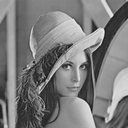
\includegraphics{128.png}
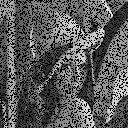
\includegraphics{0.png}
\caption{Example of a signal pair $\bs x$ (left) and $\bs y$ (right). We wish to reconstruct $\bs x$ from $\bs y$.}
\end{figure}

For example, in \cite{pilikos2014}, the signal of interest $\bs x$ is an image, so that $N$ is equal to the total number of pixels in the image and $x_i$ is equal to the intensity of the corresponding pixel.
However, we imagine that we have only access to a corrupted version of $\bs x$ in which random pixel values have been deleted.
This is our measurement $\bs y$. See Figure \ref{fig:lenna} for an example.
The sensing matrix $\bs\Omega$ corresponding to this scenario is obtained by taking the $N\times N$ identity matrix and deleting the rows that correspond to the missing entries in $\bs x$.

Compressive Sensing (CS) is a collection of signal processing techniques that allow for efficient \emph{reconstruction} (and indeed \emph{aquisition}) of such signals by solving the underdetermined system (\ref{eqn:CS}).

Of course, there are infinitely many solutions to an underdetermined system.
In the CS framework, we seek to find a solution $\hat{\bs x}$ that is \emph{sparsest in some domain}.
By that, we mean that we want to find $\hat{\bs x}$ that satisfies (\ref{eqn:CS}), such that there exists a basis transformation of $\hat{\bs x}$ in which it has the smallest number of nonzero entries.

More concretely, we assume there exists a domain in which the desired signal $\bs x$ is sparse. 
I.e. there exists a $N\times N$ basis matrix $\Psi$ such that $\bs x = \bs\Psi \bs w$ and $\bs w$ is sparse.

The CS problem can then be expressed as follows:
\begin{equation}
\label{eqn:CSproblem}
\min||\bs w||_0 \qquad\mbox{subject to}\qquad \bs\Omega\bs\Psi\bs w = \bs y
\end{equation}
where $||.||$ denotes the $l_0$ norm, i.e. the number of nonzero components.

For a more detailed review of the CS framework, see \cite{candes2008}.

\section{Wavelets Basis Transformation}
The second building block is the basis transformation
\begin{equation}
\bs x = \bs \Psi \bs w
\end{equation}
that takes the dense signal $\bs x$ and sends it into a domain in which its transformation $\bs w = \bs \Psi^T \bs x$ is sparse.

Finding a set of basis functions $\bs\Psi$ that achieve such a transformation lies at the heart of many lossy compression techniques.
For instance, in image processing the JPEG 2000 standard is a widely used lossy compression technique that relies on this principle.
The original image $\bs x$ is transformed into $\bs w$ using the so-called \emph{Discrete Cosine Transform}.
The basis matrix $\bs \Psi$ is orthogonal, so $\bs x$ and $\bs w$ have the same $l_2$ norm.
In the original signal $\bs x$ the length is spread across many of its coefficients.
On the other hand, most of the length of $\bs w$ is concentrated in a few of its coefficients.
A large fraction of the entries in $\bs w$ are very close to zero. 
By deleting these entries in $\bs w$ and only storing the non-zero coefficients (and the corresponding basis functions), we can obtain a compressed version $\hat{\bs w}$. 
This allows us to significantly reduce the amount of data that needs to be stored without affecting the visual quality in the reconstructed image $\hat{\bs x} = \bs\Psi\hat{\bs w}$.

It is important to note here that the choice of basis functions $\bs \Psi$ typically has a significant effect on the performance of the reconstruction algorithms.

The simplest wavelet basis transformation is based on the Haar wavelets.
Figure \ref{fig:haarlenna} vizualises a basis transformation of the original image $\bs x$ to $\bs w$. 
This example uses a Haar wavelet basis at the first scale.
We will explain the Haar wavelet transformations of images and videos in more detail in the next chapter.
Dark areas correspond to small coefficients.
Note that most entries in $\bs w$ are near zero. 
In practice, we approximate these entries as zero and treat $\bs w$ as sparse.

\begin{figure}
\label{fig:haarlenna}
\center
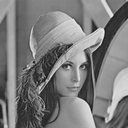
\includegraphics{128.png}
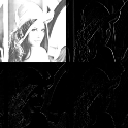
\includegraphics{haar.png}
\caption{Original image $\bs x$ (left) and its Haar basis transformation $\bs w$ (right). See next chapter for more details on Haar wavelets.}
\end{figure}

For a deeper introduction into wavelets see \cite{stollnitz1995}.
For more information on wavelet compression techniques, see \cite{devore1992}.

\section{Sparse Bayesian Learning}
So far, we have not addressed the central question: How do we solve the compressive sensing problem (\ref{eqn:CSproblem})?
Various deterministic approaches have been developed in recent years.
See \cite{pilikos2014} for an overview.

In the MPhil project, we will employ a probabilistic technique based on Sparse Bayesian Learning.
In particular, we will use the \emph{Relevance Vector Machine (RVM)} \cite{tipping2001,tipping2003} to reconstruct $\bs w$ from the measurements $\bs y$.
Following that, we obtain a reconstructed version of the desired signal $\bs x$ by pre-multiplying $\bs w$ by $\bs \Psi$ to obtain the desired signal.

The RVM is a \emph{regression} technique.
We model the relationship between $\bs y$ and $\bs x$ by
\begin{equation}
\label{eqn:rvmmodel}
y_i = \bs w^T \bs \psi(x_i) + \epsilon_i
\end{equation}
where $\psi(x_i)$ is the $i$th column of $\Psi$ and the $\epsilon_i$ are independent noise variables drawn from a zero-mean Gaussian distribution $\mathcal{N}(o,\sigma^2)$.

The model uses the available measurements $\{(x_1,y_1),\dots,(x_M,y_M)\}$ as training data to train the model in a Bayesian framework.
The result of training the RVM is a posterior distribution for the unknown vector of coefficients $\bs w$.
A special feature of the RVM is that the posterior mean $\bs \mu$ of $\bs w$ is often very sparse.

In order to reconstruct the image, we use the estimated posterior mean to ``predict'' what a pixel value $y^*$ should be at a location $x^*$ in which information was missing:
\begin{equation}
y^* = \bs w^T\bs\psi(x^*)
\end{equation}

\begin{figure}
\label{fig:lennareconstruction}
\center
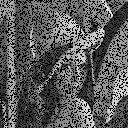
\includegraphics{0.png}
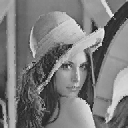
\includegraphics{3.png}
\caption{Corrupted signal $\bs y$ (left) and reconstructed signal $\hat{\bs x}$ (right) using a cascade of 3 RVMs with Haar basis functions (see \cite{pilikos2014}).}
\end{figure}

Apart from achieving sparse solutions, one further desirable feature of the RVM is that the model provides error bars for its predictions.
This is used in \cite{pilikos2014} to construct a multi-scale cascade of RVM estimations and achieve significant performance boosts.

An example of this can be seen in Figure \ref{fig:lennareconstruction}.

For details on the RVM and its implementation see \cite{pilikos2014,tipping2003,tipping2001}.


\chapter{Current Implementation}
This chapter gives a brief description of the current state of our implementation of the 3D signal reconstructer.

\section{Code Review}
Our implementation is based on the work in \cite{pilikos2014}.
As such, approximately one week was spent reviewing his code base in order to become familiar with code and also to look for possible bugs.
Although two minor bugs were discovered, fixing them had no qualitative effect on the output of the code.

\section{Haar basis functions}
The RVM takes as input a target vector ($\bs y$) and a basis matrix ($\bs \Psi$). 
In this respect, it is agnostic about whether the signal is an image or video or of some other type alltogether.
Most of this information is encoded in the basis matrix $\bs \Psi$.
It is therefore important, and often challenging, to select a good set of basis functions.

Our current implementation uses 3-dimensional Haar wavelet basis functions.
I will show how the basis matrix $\bs\Psi$ is constructed by briefly describing how the discrete Haar wavelet transform is performed on 1D, 2D and finally on 3D signals.

\subsection{1D Haar wavelet transform}
Consider a 1-dimensional signal $\bs s = \{s_1,\dots,s_r\} \in \mathbb{R}^r$ ($r$ for ``rows''), where, for simplicity, we assume that $r$ is a power of 2.
The Haar wavelet transform can be performed at various resolution scales.
The transform at the first scale is given by:
\begin{equation*}
\bs s = \{s_1,\dots,s_r\}\to \frac{1}{\sqrt{2}}\{s_1+s_2,s_3+s_4,\dots,s_{r-1}+s_r,s_1-s_2,\dots,s_{r-1}-s_r\}=\hat{\bs s}^{(1)}
\end{equation*}
The first half of the signal is replaced by scaled averages of adjacent elements and the second half is replaced by scaled differences of adjacent elements.
By performing this transform again on the first half of $\hat{\bs s}^{(1)}$ while keeping the second half fixed, we get the Haar wavelet transform at the second scale $\hat{\bs s}^{(2)}$. 
To get the third scale transform $\hat{\bs s}^{(3)}$, we perform the initial transform on the first quarter of $\hat{\bs s}^{(2)}$ while keeping the rest of the signal fixed.
We may continue this process until we reach the $i$th scale, where $2^i = r$.

From here on, we will only consider the first scale transform $\hat{\bs s}^{(1)}$ and we will omit the $(1)$ superscript.
We can express the transform as a multiplication by an orthogonal $r\times r$ matrix $W$ given by
\begin{equation}
W = \begin{bmatrix}
  \Phi_r \\
  \Psi_r \\
\end{bmatrix}
\end{equation}
where $\Phi_r$ and $\Psi_r$ are $(r/2)\times r$ matrices\footnote{Note that the matrix $\Psi_r$ used here is different to the matrix $\Psi$ that was used in the previous chapter (which corresponds to $W^T$ here).} given by
\begin{equation*}
\Phi_r = \frac{1}{\sqrt{2}} \begin{pmatrix}
1&1&0&0&\cdots&0&0\\
0&0&1&1&\cdots&0&0\\
\vdots&\vdots&\vdots&\vdots&\ddots&\vdots&\vdots\\
0&0&0&0&\cdots&1&1
\end{pmatrix}
\end{equation*}
and 
\begin{equation*}
\Psi_r = \frac{1}{\sqrt{2}} \begin{pmatrix}
1&-1&0&0&\cdots&0&0\\
0&0&1&-1&\cdots&0&0\\
\vdots&\vdots&\vdots&\vdots&\ddots&\vdots&\vdots\\
0&0&0&0&\cdots&1&-1
\end{pmatrix}
\end{equation*}


In the signal processing literature, $\Phi_r$ is referred to as a low pass filter, while $\Psi_r$ is referred to as a high pass filter.
$\Phi_r$ outputs an average of the signal and $\Psi_r$ outputs the details of the signal.

\subsection{2D Haar wavelet transform}
Let $A \in \mathbb{R}^{r\times c}$ be a 2-dimensional signal (e.g. an image).
For simplicity, we will assume that both $r$ and $c$ are powers of 2 (though not necessarily equal).

It is simple to obtain $A$'s Haar wavelet transform $\hat{A}$ at the first scale.
This is done by first applying the 1-dimensional transform individually to each column of $A$ to obtain a temporary matrix $\hat A_{temp}$.
Next, we apply the 1-dimensional haar wavelet transform individually to each row of $\hat A_{temp}$ to obtain $\hat A$.

We can again express the transform as a multiplication of matrices:
\begin{equation}
\label{eqn:2Dtransform}
\hat A = \begin{bmatrix}
  \Phi_r\\
  \Psi_r\\
\end{bmatrix}
A
\begin{bmatrix}
  \Phi_c^T & \Psi_c^T\\
\end{bmatrix}
\end{equation}
where $\Phi_r$ and $\Psi_r$ are as before and $\Phi_c$ and $\Psi_c$ are of similar form but each have dimensions $(c/2)\times c$.
This is the transform that was used to generate the RHS of Figure \ref{fig:haarlenna}.
We note that the high-pass filters essentially detect edges of various orientations in the image.

However, as it currently stands, we cannot use this form of the basis transformation for the reconstruction algorithm. Recall that the RVM requires a \emph{vector} of measurements as opposed to a matrix and also that it requires a single basis matrix, not a basis transform as given in (\ref{eqn:2Dtransform}).

To do this, we store the 2-dimensional signal $A$ as a long column vector $\bs a$ of length $rc$ by pasting the individual columns of $A$ one after another.
The basis transformation of $\bs a$ can then be expressed as 
\begin{equation*}
\hat{\bs a} = W \bs a
\end{equation*}
where $W$ is a $rc \times rc $ matrix given by
\begin{equation*}
W = 
\begin{bmatrix}
\Phi_c \otimes \Phi_r \\
\Phi_c \otimes \Psi_r \\
\Psi_c \otimes \Phi_r \\
\Psi_c \otimes \Psi_r \\
\end{bmatrix}
\end{equation*}

The symbol $\otimes$ denotes the \emph{Kronecker product}. 
The kronecker product $P \otimes Q$ between matrices $P$ and $Q$ with dimensions $m_P \times n_P$ and $m_Q \times n_Q$, respectively,  is defined to be the block matrix
\begin{equation*}
\begin{bmatrix}
p_{1,1} Q & p_{1,2} Q & \cdots & p_{1,n_P} Q \\
p_{2,1} Q & p_{2,2} Q & \cdots & p_{2,n_P} Q \\
\vdots&\vdots&\ddots&\vdots \\
p_{m_P,1} Q & p_{m_P,2} Q & \cdots & p_{m_P,n_P} Q \\
\end{bmatrix}
\end{equation*}
of size $m_Pm_Q \times n_Pn_Q$.

\subsection{3D Haar wavelet transform}
Let $V \in \mathbb{R}^{r\times c\times s}$ be a 3-dimensional signal such as a video. 
$V$ has $r$ rows, $c$ columns and $s$ slices, and we assume that $r$, $c$ and $s$ are all powers of 2. 
We may visualize $V$ as a ``volume'' with 2 spacial dimensions and one time dimension corresponding to frames of the video.

To obtain the Haar wavelet transform $\hat V$ of $V$, we first perform the 1-dimensional transform individually on each column in every slice of $V$ to get $\hat V_{temp1}$.
We then perform the 1D transform on every row in every slice of $\hat V_{temp_1}$ to get $\hat V_{temp_2}$.
Finally, we perform the 1D transform across the slices for every row and column to get $\hat V$.

However, like in the 2-dimensional case, we need to be able to pass a single vector of coefficients and a single basis matrix to the RVM.
To do this, we vectorize $V$ as follows. 
First, we vectorize each individual slice of $V$ as before in the 2D case.
Then, we stack all these vectors on top each other to get one very long column vector $\bs v$ of length $rcs$.
The Haar wavelet transform is given by 
\begin{equation*}
\hat{\bs v} = W \bs v
\end{equation*}
where 
\begin{equation*}
W = 
\begin{bmatrix}
\Phi_s \otimes \Phi_c \otimes \Phi_r \\
\Phi_s \otimes \Phi_c \otimes \Psi_r \\
\Phi_s \otimes \Psi_c \otimes \Phi_r \\
\Phi_s \otimes \Psi_c \otimes \Psi_r \\
\Psi_s \otimes \Phi_c \otimes \Phi_r \\
\Psi_s \otimes \Phi_c \otimes \Psi_r \\
\Psi_s \otimes \Psi_c \otimes \Phi_r \\
\Psi_s \otimes \Psi_c \otimes \Psi_r \\
\end{bmatrix}
\end{equation*}
Comparing notation to the previous chapter, what we refer to as $W$ here is the transpose of what was previously denoted as $\Psi$.
And since $\bs v = W^T \hat{\bs v}$, we see that $\bs v$ corresponds to what was previously called $\bs x$. 

\section{Preliminary Results from first working Prototype}
We have obtained some results with our current implementation.
The implementation uses the Haar wavelet transform at the first scale.

Our example video has a resolution of 128 by 128 pixels and consists of a total of 64 frames.
Thus, $r = 128$, $c = 128$ and $s = 64$.
Note that even for such a relatively small sample, the size of the basis matrix $\Psi$ is $(128*128*64)\times(128*128*64) = 1048576\times 1048576$.
Even in single precision, storing this matrix would require around 4 terrabytes.

For this reason, we have split the original input signal into $8\times 8\times 8$ blocks and perform the algorithm on the individual blocks.
\begin{figure}
\label{fig:foreman}
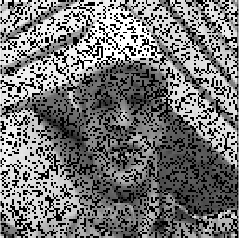
\includegraphics{corr.png}
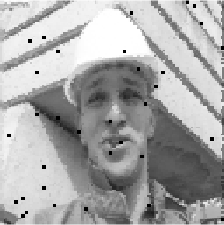
\includegraphics{rec.png}
\caption{Sample frame from corrupted video (left) and the reconstructed video (right)}
\end{figure}

\begin{figure}
\label{fig:soccer}
\center
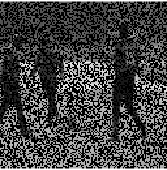
\includegraphics{corr2.png}
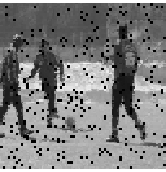
\includegraphics{rec2.png}
\caption{Sample frame from corrupted video (left) and the reconstructed video (right)}
\end{figure}

In Figures 3.1 and 3.2, we have included a sample frame from the corrupted test video and the same frame after reconstruction.

In Figure 3.1, we corrupted the video by deleting 30\% of the pixel values in the first frame and deleting the same pixel values in each subsequent frame (so the same pixels are missing in each frame).
Figure 3.2 uses the same corruption scheme but we deleted 50\% rather than 30\% of pixel values.

These initial results are promising, though clearly there are still improvements to be made.

\chapter{Still To Do}

\section{Software Development}
\subsubsection{Multi-Scale Haar wavelets}
Currently, the code uses Haar basis functions at the first scale. 
Note how in the reconstructed videos in Figures \ref{fig:foreman} and \ref{fig:soccer}, there are still missing (black) patches.
Using Haar basis functions at higher scales allows us to fill these missing areas.

\subsubsection{Cascade of Estimations}
Using higher scales of the Haar wavelets often results in somewhat blurry reconstructions.
The image reconstruction algorithm in \cite{pilikos2014} employs a cascade of estimations.
By using Haar wavelets at multiple scales in a cascade, we are able to achieve sharper reconstructions while also filling all the missing pixel values and frames.

The cascade will be the next addition to the current prototype.

\subsubsection{Discrete Cosine Transform}
Once the Haar wavelets and the cascade have been implemented, I would like to explore the use of the Discrete Cosine Transform as a choice of basis transformation. 
There are potentially quite significant performance gains.

\subsubsection{Strengthening the code base}
It may be worth spending some time in making the code base more robust.
For example by moving the code to an object-oriented design or at least by adding a debug mode and some unit tests.

\subsubsection{Parallel Implementation}
The signal is typically broken into distinct patches which get processed independently of one another.
Parallelizing the code (e.g. by using MPI or CUDA) would likely to significant speed-ups.

\section{Dissertation}
\subsubsection{Extensive Literature Review}
A significant part of the project will be an extensive review on the current literature in the field of video reconstruction and video encoding.
A more extensive review of the Compressive Sensing framework may also be included here as well as, potentially, the theory of wavelets. 


\subsubsection{Performance Analysis}
There are two parts to this. First, how is the performance affected by different settings of the parameters of the algorithm.
Secondly, how does our method compare to other existing signal reconstruction methods? Under what circumstances we get superior performance? How could we improve the method?

\section{Schedule}
Having implemented a first working prototype, I believe we are well on schedule to finish on time.
The plan is to have a first draft ready by mid July.
The next page gives a rough outline of the schedule in form of a Gantt chart.

%\setboolean{@twoside}{false}
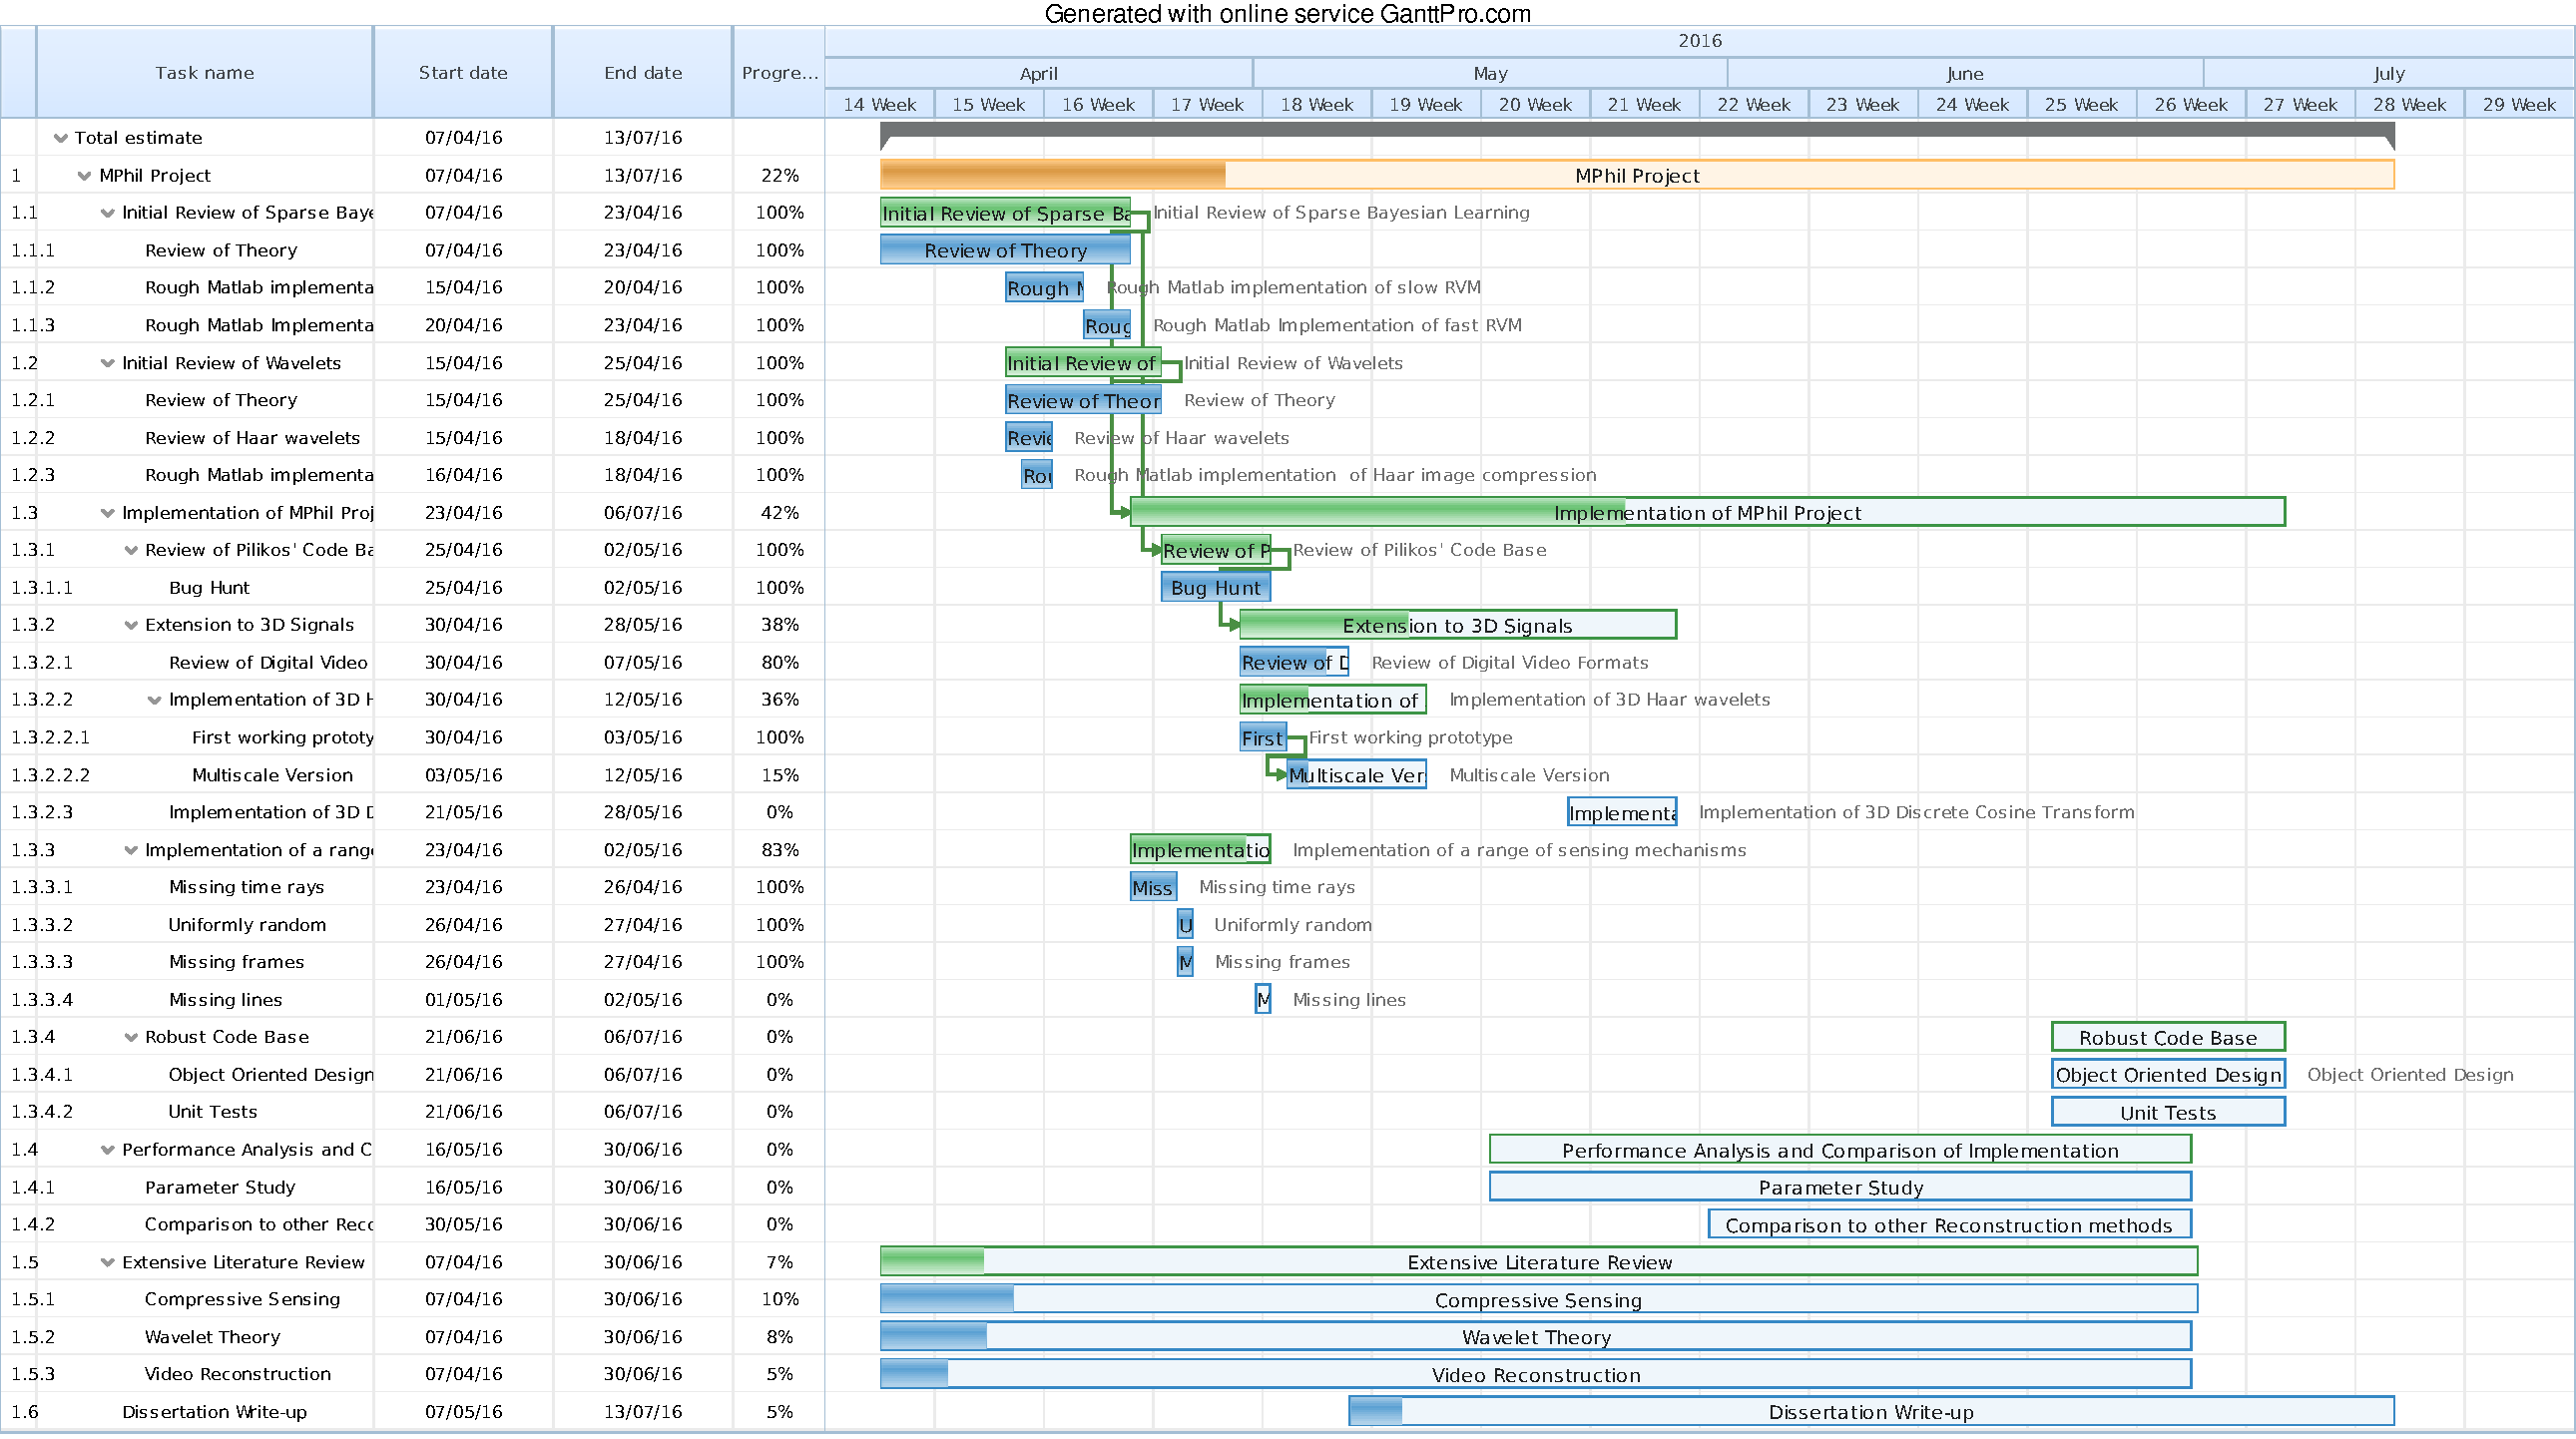
\includepdf[pages={1},angle=270]{gantt.pdf}
%\section*{Acknowledgements}
%Here I acknowledge the assistance of my supervisor, my industrial sponsor,
%and the effects of caffeine on my ability to produce this report on time.

%% The Appendices part is started with the command \appendix;
%% appendix sections are then done as normal sections
%\appendix

%% References
%%
%% Following citation commands can be used in the body text:
%% Usage of \cite is as follows:
%%   \cite{key}         ==>>  [#]
%%   \cite[chap. 2]{key} ==>> [#, chap. 2]
%%

%% References with bibTeX database:
%\section*{Bibliography}
\bibliographystyle{elsarticle-num}
%\bibliographystyle{apa}
\bibliography{referencesRVM.bib}

%% Authors are advised to submit their bibtex database files. They are
%% requested to list a bibtex style file in the manuscript if they do
%% not want to use elsarticle-num.bst.

%% References without bibTeX database:

% \begin{thebibliography}{00}

%% \bibitem must have the following form:
%%   \bibitem{key}...
%%

% \bibitem{}

% \end{thebibliography}


\end{document}

%%
%% End of file `rvm.tex'.